\documentclass[a4paper, 12pt]{article}


%%%%%%%%%%%%
% Packages %
%%%%%%%%%%%%

\usepackage[english]{babel}

\usepackage[noheader]{sleek/sleek}
\usepackage{sleek/sleek-title}


%%%%%%%%%%%%%%%%%%%%%%%
% Title page settings %
%%%%%%%%%%%%%%%%%%%%%%%

\logo{resources/pdf/logo-uliege.pdf}
\institute{University of Liège}
\title{Project 4 : Drawing the fork primitive}
\subtitle{Operating systems}
\author{
    Maxime \textsc{Meurisse} (s161278)\\
    Valentin \textsc{Vermeylen} (s162864)\\
}
\context{Master in Engineering and Computer Science}
\date{Academic year 2019-2020}


%%%%%%%%%%%%%%
% References %
%%%%%%%%%%%%%%

\addbibresource{references.bib}


%%%%%%%%%%%%
% Document %
%%%%%%%%%%%%

\begin{document}
    % ----- Title page ----- %
    
    \maketitle
    
    % ----- Introduction ----- %
    
    \section{Introduction}
    
    In the context of the version of Linux installed on the course reference virtual machine (Linux 4.15)\footnote{All explanations in this document will refer to this version of Linux.}, \emph{fork} is an operation that allows a process to create a copy of itself. This operation is usually used in combination with the system call \emph{exec} so that the newly created process, called \emph{child process}, can execute another operation.
    
    An important point of the fork operation is \emph{memory management}. This document highlights first the different major operations taking place in the Linux kernel when calling a fork and then how the memory, and more specifically that of the child process, is managed.
    
    The various explanations are supported by a diagram presented in the appendix of this document and also attached as a \texttt{diagram.pdf} file.
    
    % ----- Implementation ----- %
    
    \section{Implementation}
    
    The fork system call is not implemented in \emph{sys\_call} any longer. It actually calls the \emph{clone} function (a system call to create a new thread) which itself calls the \emph{\_do\_fork} function that does the work of creating a new process. The latter is the actual implementation of the fork operation. It calls the function \emph{copy\_process} which performs all the main operations to create the new process.
    
    \subsection{Main operations}
    
    Main operations performed by the function \emph{copy\_process} are listed below.
    
    \begin{enumerate}
        \item \emph{The copy\_process function} : this function creates a new process as a copy of the parent, but does not start it. It copies the registers and the appropriate parts of the process environment, but the starting of the new process is left to the caller.
        
        The function first checks that the flags passed as parameters are compatible, then calls the function \emph{dup\_task\_struct}.
        
        \item\label{memory.step} \emph{The dup\_task\_struct function} : this function is used to create new kernel stacks for the new thread that is being created, as well as allocate the \emph{task\_struct} used to represent the new process (this structure is used to store a lot of state information), and the \emph{thread\_info} structure. All those values are the same as the ones of the parent process (the origin of the call to fork).
        
        After that, process descriptor are cleared or set to initial values. It also sets the usage counter of the new \emph{task\_struct} to 2 so that the operating system knows the corresponding process is alive and not dead or in a zombie or orphan state.
        
        A function \emph{copy\_flags} is called to update the flags member of the \emph{task\_struct} structure. Depending on the flags, what resources are to be shared is decided.
        
        Finally, that data structure is returned at the end of the function.
        
        \item \emph{End of copy\_process} : once the task structure has been allocated and correctly filled, a return stack is allocated to the newly created task. The function then goes to set all fields of the newly created structure appropriately and returns to the caller a pointer to the newly created child.
        
        \item \emph{Coming back to \_do\_fork} : finally, after checks to see if the new thread pointer is not invalid, the process is awoken.
    \end{enumerate}
    
    It is in step \ref{memory.step} that the main elements of the child process are allocated and copied from the parent process. The different memory management mechanisms are presented in the next section.
    
    % ----- Memory management ----- %
    
    \section{Memory management}
    
    \subsection{Overview}
    
    When the fork operation is called, it creates a new address space for the child process. In theory, the two processes therefore work in two distinct address spaces and therefore whatever operation is performed by one process will not affect the other process.
    
    As mentioned in step \ref{memory.step} of the implementation, it is the \emph{task\_struct} structure that is copied. This structure is called a \emph{Process Control Block} (PCB). It contains a lot of state information : pid, user id, register state, process status, etc. Not all fields in the structure are strictly copied; some, such as pid or process status, are obviously not copied from the parent. All the memory segments of the parent process is also duplicated. These two elements (memory and PCB) characterize a process in the kernel.
    
    In practice, this would mean copying a lot of memory elements each time an exec is called by a child process created with fork. To avoid this, Linux uses a technique called \emph{Copy-on-write} (COW) : the parent and child processes share a single copy of the process address space and only when one of them tries to write into the process address space, a new copy is created for that process.
    
    This technique avoids copying large segments of memory each time an exec is called by a child process.
    
    \subsection{Copy-on-write}
    
    Copy-on-write is a technique to efficiently copy data resources in a computer system. The principle is as follows : when a resource is duplicated but not modified, it is not necessary to create a copy. As the name of the technique suggests, a copy is created only when a write to memory is performed.
    
    It can be implemented efficiently by using the page table : the pages of memory of the parent process are marked as read-only and the kernel keeps a count of the number of references to the page.
    
    If both processes only read, they work with shared memory, but when a process (parent or child) tries to write to one of these pages, it creates a \emph{page fault} which is intercepted by the kernel trap handler. The latter then creates a new physical page (except if there is only one reference to this page), changes the permission in \emph{read-write}, updates the page table, decrements the number of references and returns the \emph{Program Counter} (PC) to the previous statement. The latter is then re-run and the writing in memory (on the newly created page) can be done.
    
    Thanks to this new allocated page, a change made in one process will not be visible in another.
    
    \subsection{Cases of failure}
    
    The fork operation can fail in some situations. Concerning memory, the operation may fail if no more memory is available (\emph{out of memory}) or if the parent process consumes more than 50\% of the system memory.
    
    In the latter case, the creation of the child process would not be especially problematic (since not all the memory of the parent process is directly copied) but the interaction with the elements of the memory by the child process would be problematic (the elements would then be copied by the COW mechanism but would in fact not have enough memory to be copied).
    
    \subsection{File descriptor}
    
    As mentioned in step \ref{memory.step} of the implementation, process descriptors are cleared and set to initial values. However, the file descriptor of the parent is not duplicated when the child process is created. This implies that resources can be shared between the different processes. Some anonymous objects (pipes, shared memory, etc.) can only be shared through this mechanism.
    
    % ----- Appendix ----- %
    
    \newpage
    \appendix
    \section*{Diagram}
    
    The diagram is shown in Figure \ref{fig:diagram.fork}.
    
    \begin{figure}[H]
        \centering
        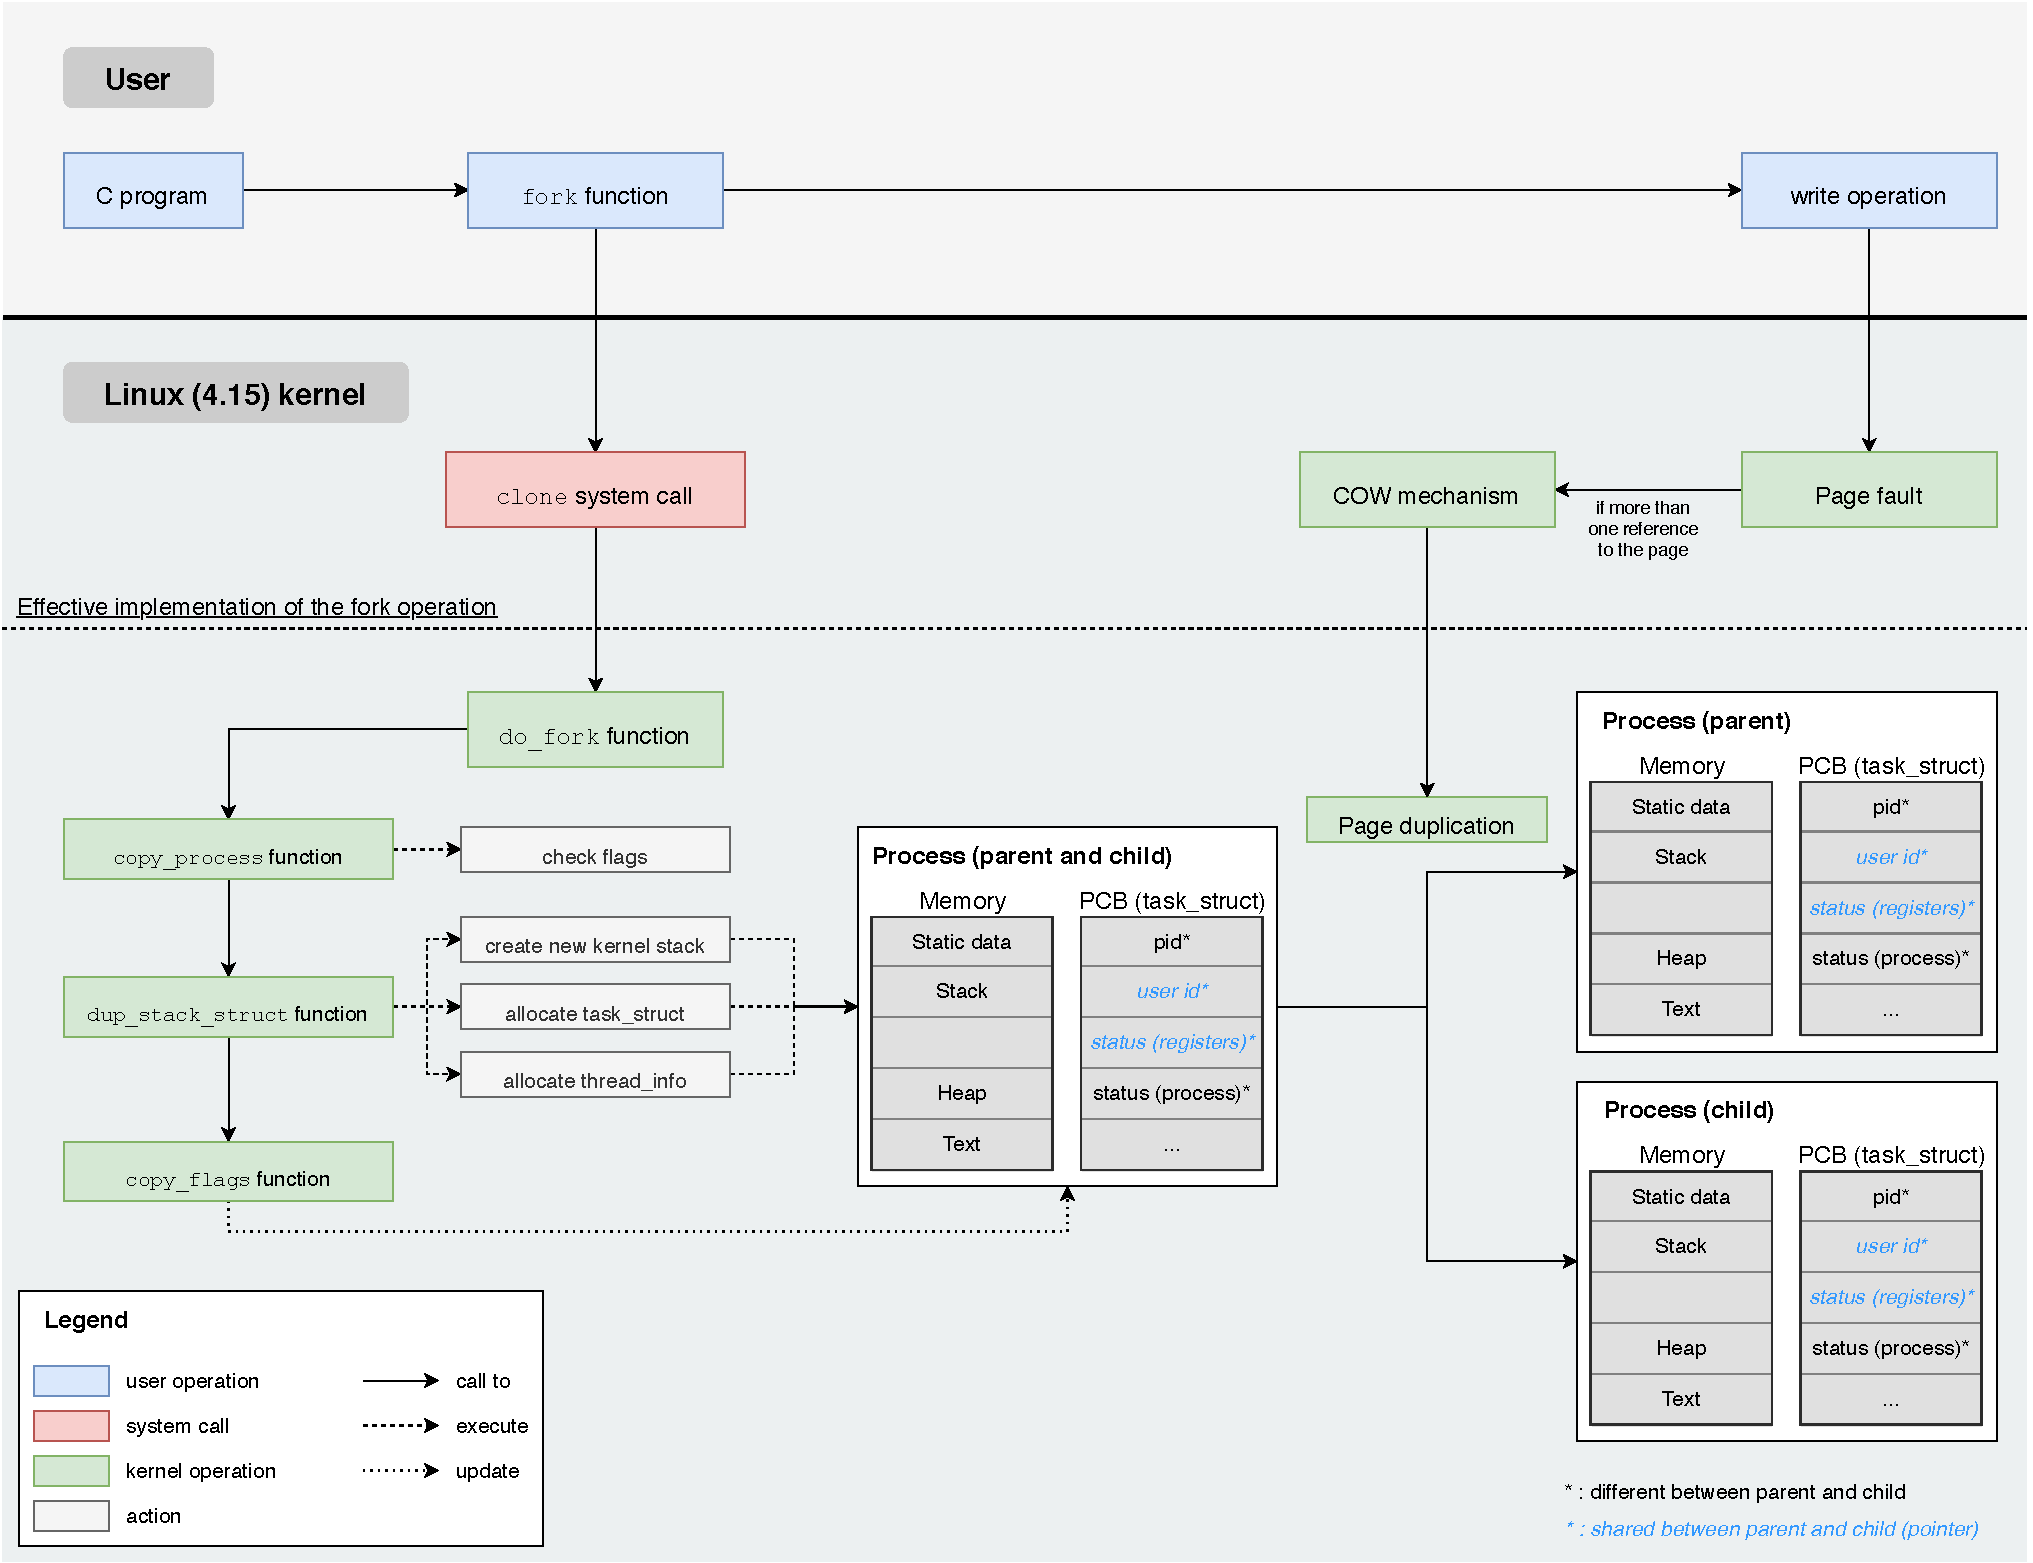
\includegraphics[width=\textwidth]{resources/pdf/diagram.pdf}
        \caption{Diagram of the fork operation in the Linux kernel.}
        \label{fig:diagram.fork}
    \end{figure}
    
    % ----- References ----- %
    
    \newpage
    \nocite{*}
    \printbibliography
\end{document}
